\documentclass[11pt]{article}

\usepackage[margin=1in]{geometry}
\usepackage{amsmath, amssymb}
\usepackage{graphicx}
\usepackage{booktabs}
\usepackage{float}
\usepackage{hyperref}
\usepackage{enumitem}
\usepackage{titlesec}

\setlength{\parindent}{0pt}
\setlength{\parskip}{4pt}
\setlist[itemize]{leftmargin=1.2em,itemsep=1pt,topsep=2pt}
\titlespacing*{\section}{0pt}{8pt}{4pt}
\titlespacing*{\subsection}{0pt}{6pt}{3pt}

\title{Earnings Call Sentiment Analysis for Stock Return Prediction}
\author{Nikita Mehendale \and Charles Wu \and Ruoyang Li \and Patrick Pham \and Nathaniel Kung \and Prabhav Pagadala}
\date{May 11, 2026}

\begin{document}

\maketitle

\begin{abstract}
This project studies whether deep learning models can use earnings call transcripts to predict short-term stock movement after an earnings announcement. We formulate the problem as supervised three-class classification, where the model takes an earnings call transcript as input and predicts whether the post-open abnormal return is down, flat, or up. Our current pipeline uses a local transcript dataset, matches each call to stock return data, assigns labels using a $\pm 0.5\%$ flat band, and converts each transcript into overlapping FinBERT token chunks. We implement two transformer-based models: a FinBERT baseline that mean-pools chunk embeddings and a hierarchical transformer that applies second-level self-attention across transcript chunks. This report describes our current data pipeline, model design, training setup, and expected evaluation plan. Final training curves, metrics, and error analysis will be inserted after the remaining experiments are completed. \textbf{TODO: Add one sentence with final best model, test accuracy, macro F1, and main takeaway.}
\end{abstract}

\section{Introduction and Motivation}

Earnings calls are a useful setting for applying deep learning to real financial text because they contain both structured business discussion and unstructured language from managers and analysts. After a company reports quarterly results, management usually discusses revenue, margins, guidance, risks, and future demand. Investors may react not only to the numerical earnings release, but also to how management explains the quarter and answers analyst questions. This makes earnings call transcripts a natural source of qualitative information for predicting post-earnings stock movement.

Our project asks whether a neural text model can learn a relationship between transcript language and the stock's post-earnings abnormal return. The use case is not to build a fully automated trading system, but to study whether domain-specific NLP can extract signal from a noisy, real-world financial prediction task. This is a challenging learning problem because earnings calls are long documents, the language is specialized, and the label is affected by many things outside the transcript, including market expectations, macro news, sector movement, and information already priced into the stock.

The main research question is: \textit{Can FinBERT-based deep learning models predict whether a stock's post-open abnormal return after an earnings call will be down, flat, or up?} We compare a simpler FinBERT mean-pooling baseline with a hierarchical transformer that is designed for long transcript classification. Our contribution is a complete supervised learning pipeline that turns raw earnings call transcripts into tokenized model inputs, constructs return-based class labels, trains transformer-based classifiers, and evaluates whether hierarchical self-attention across transcript chunks improves the prediction task.

\section{Data and Learning Problem}

\subsection{Dataset and Features}

Our current raw transcript set contains 1,185 text files. After applying the current filename parser and the configured date range of 2017 through 2024, 1,119 transcripts remain across 48 tickers. The average transcript length is about 18,790 words, with a median of 18,176 words. This confirms that the data is a long-document NLP problem rather than a short sentence-level sentiment task.

Each transcript is used as the feature input $X_i$. Since earnings call transcripts are much longer than the input length of a standard BERT-style model, we split each transcript into overlapping token chunks. The current preprocessing uses 450 tokens per chunk, a 50-token overlap, and a maximum of 32 chunks per transcript. For transcript $i$, the model input can be written as
\[
X_i = \{x_{i1}, x_{i2}, \ldots, x_{iC_i}\},
\]
where $x_{ic}$ is chunk $c$ from transcript $i$ and $C_i$ is the number of chunks retained for that transcript. Each chunk also has an attention mask so padded tokens do not affect the transformer output.

\subsection{Label Construction}

The label is based on post-open abnormal return. We use the next market open after the call as the start of the return window, rather than focusing on the overnight gap. The current return script computes a post-open return and subtracts the corresponding SPY return over the same window to create an abnormal return. Let $r_i$ be the abnormal return for call $i$. We convert it into a three-class label:
\[
Y_i =
\begin{cases}
0, & r_i < -0.005 \quad \text{(down)}, \\
1, & -0.005 \leq r_i \leq 0.005 \quad \text{(flat)}, \\
2, & r_i > 0.005 \quad \text{(up)}.
\end{cases}
\]
The flat class is important because a very small abnormal return should not necessarily be treated as a meaningful positive or negative market reaction.

\subsection{Preprocessing and Data Quality}

The pipeline has four main steps. First, local transcript text files are converted into a normalized JSON format. Second, stock and SPY prices are downloaded around each call date. Third, abnormal returns are calculated and converted into down, flat, and up labels. Fourth, the transcript text is tokenized and chunked for the PyTorch dataset class. The dataset interface returns token chunks, attention masks, labels, tickers, and call dates.

There are a few data quality issues that matter for the final interpretation. Transcript files are not perfectly standardized, and some filenames with non-standard ticker symbols are skipped by the current parser. More importantly, the local transcript filenames provide year and quarter, so the current local loader uses a quarter-based proxy date. This is enough to build and test the pipeline, but exact earnings call dates should be verified before making a strong claim about financial predictive performance. The final report should also include the class balance after return labels are generated because class imbalance could make accuracy misleading.

\begin{table}[H]
\centering
\begin{tabular}{lcc}
\toprule
Dataset item & Current value & Final value to confirm \\
\midrule
Raw transcript text files & 1,185 & 1,185 \\
Usable transcripts after parser/date filter & 1,119 & TODO \\
Unique tickers after parser/date filter & 48 & TODO \\
Average transcript length & 18,790 words & TODO \\
Flat band for labels & $\pm 0.5\%$ & $\pm 0.5\%$ \\
Train/validation/test split & 70/15/15 chronological & TODO counts \\
\bottomrule
\end{tabular}
\caption{Current dataset summary. Final values may change after exact date matching and return filtering.}
\label{tab:data-summary}
\end{table}

\begin{figure}[H]
\centering
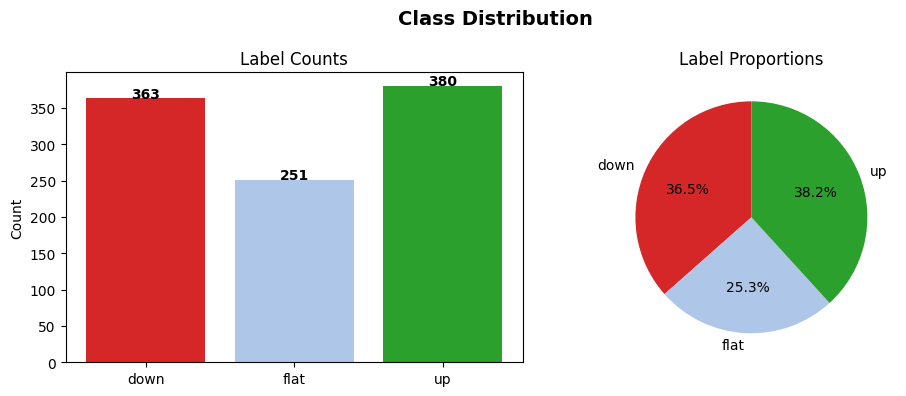
\includegraphics[width=0.9\textwidth]{images/class_distribution.png}
\caption{Class distribution of the three return-based labels after applying the $\pm 0.5\%$ flat band. The up (38.2\%) and down (36.5\%) classes are similarly represented, while the flat class (25.3\%) is somewhat smaller, which motivates reporting macro F1 in addition to accuracy.}
\label{fig:class-distribution}
\end{figure}

\begin{table}[H]
\centering
\small
\begin{tabular}{lccccl}
\toprule
Split & Count & Down & Flat & Up & Date range \\
\midrule
Train & 695 & 263 & 176 & 256 & 2017-12-01 $\rightarrow$ 2022-09-01 \\
Validation & 149 & 49 & 43 & 57 & 2022-09-01 $\rightarrow$ 2023-09-01 \\
Test & 150 & 51 & 32 & 67 & 2023-09-01 $\rightarrow$ 2024-12-01 \\
\midrule
Total & 994 & 363 & 251 & 380 & 2017-12-01 $\rightarrow$ 2024-12-01 \\
\bottomrule
\end{tabular}
\caption{Chronological train/validation/test split after return filtering, with per-class counts and date ranges. The split follows a roughly 70/15/15 ratio and preserves temporal ordering so that future market conditions cannot leak into the training set.}
\label{tab:splits}
\end{table}

\section{Methodology}

\subsection{Problem Formulation}

We formulate the task as supervised multiclass classification. Given transcript input $X_i$ and label $Y_i \in \{0,1,2\}$, the model learns a function $f_\theta(X_i)$ that outputs logits for the down, flat, and up classes. After applying softmax, the model produces a probability vector $\hat{p}_i \in \mathbb{R}^3$. The training objective follows the standard empirical risk minimization form from class:
\[
\min_{\theta} \frac{1}{N}\sum_{i=1}^{N} L(f_\theta(X_i),Y_i) + R(\theta),
\]
where $L$ is cross-entropy loss and $R(\theta)$ represents regularization through dropout, weight decay, early stopping, and partially frozen FinBERT layers.

\subsection{FinBERT Baseline}
We used FinBERT as the main text encoder for earnings call transcripts. FinBERT is a BERT-based transformer model pre-trained on financial text.
Since each transcript is much longer than the maximum sequence length accepted by BERT-style models, we split each transcript into overlapping chunks of 450 tokens with an overlap of 50 tokens. Each chunk was independently passed into FinBERT. For each chunk, we used the final hidden representation of the \texttt{[CLS]} token as the chunk-level embedding:
\[
h_j = \mathrm{FinBERT}(x_j)_{\texttt{[CLS]}}
\]
where \(x_j\) is the \(j\)-th chunk of a transcript and \(h_j \in \mathbb{R}^{768}\) is its FinBERT representation.
To reduce overfitting and avoid catastrophic forgetting, we froze the first 6 transformer layers of FinBERT and fine-tuned only the higher layers. This allows the model to preserve general financial-language representations while adapting to our specific stock movement prediction task.
\subsection{Chunk Aggregation and Prediction Head}
For the FinBERT baseline, we aggregated chunk embeddings using mean pooling across all valid chunks:
\[
h = \frac{1}{M} \sum_{j=1}^{M} h_j
\]
where \(M\) is the number of non-padding chunks in the transcript. Padding chunks were ignored during pooling.
The pooled transcript representation was then passed through a feedforward classification head:
\[
z = W_2 \cdot \mathrm{Dropout}(\mathrm{GELU}(W_1 h + b_1)) + b_2
\]
where \(z \in \mathbb{R}^{3}\) represents logits for the three classes: down, flat, and up.

\subsection{Hierarchical Transformer Model}

The main advanced component is a hierarchical transformer. The first level is the same FinBERT chunk encoder used in the baseline. The second level treats the sequence of chunk embeddings as a new sequence and applies a transformer encoder across chunks. We add a learnable chunk-level \texttt{[CLS]} token, learnable positional embeddings over chunk positions, and a two-layer transformer encoder with 8 attention heads and feedforward dimension 1024. The final chunk-level \texttt{[CLS]} output is passed through a layer-normalized classification head.

This model is appropriate because important earnings call information can appear in different locations. Prepared remarks may contain high-level guidance, while the analyst Q\&A section may reveal uncertainty or pressure that is not obvious from the opening script. Mean pooling assumes every chunk contributes in a simple average, while self-attention allows the model to learn interactions between chunks and place more weight on the parts of the transcript that are useful for prediction.

\subsection{Training Choices}

We train using cross-entropy loss:
\[
L = -\frac{1}{N}\sum_{i=1}^{N}\sum_{k=1}^{3}\mathbf{1}\{Y_i=k\}\log(\hat{p}_{ik}).
\]
The optimizer is AdamW with learning rate $2\times 10^{-5}$ and weight decay $10^{-2}$. We use dropout of 0.1, gradient clipping with maximum norm 1.0, a cosine learning rate schedule, and early stopping with patience 3. The first 6 FinBERT layers are frozen to reduce training cost and limit overfitting. The planned split is chronological: 70\% train, 15\% validation, and 15\% test. Chronological splitting is important because a random split could leak future market conditions into the training set.

\begin{table}[H]
\centering
\begin{tabular}{lc}
\toprule
Hyperparameter & Value \\
\midrule
FinBERT model & \texttt{ProsusAI/finbert} \\
Chunk size / overlap & 450 / 50 tokens \\
Maximum chunks per transcript & 32 \\
Hidden dimension & 768 \\
Hierarchical transformer layers & 2 \\
Attention heads & 8 \\
Dropout & 0.1 \\
Batch size & 16 \\
Learning rate & $2\times 10^{-5}$ \\
Weight decay & $10^{-2}$ \\
Maximum epochs / patience & 10 / 3 \\
\bottomrule
\end{tabular}
\caption{Model and training hyperparameters.}
\label{tab:hyperparameters}
\end{table}

\section{Experimental Setup and Results}

The codebase is organized into separate modules for data loading, preprocessing, model definitions, training, evaluation, utilities, and the demo. We track experiments with Weights \& Biases and save the best checkpoint according to validation loss. The evaluation code reports accuracy, macro F1, weighted F1, up-class F1, down-class F1, and a confusion matrix. Macro F1 is especially important because the flat, up, and down classes may not be balanced.

At the time of this draft, the pipeline and model code are implemented, but the final training runs and plots still need to be added. The results section should be completed once the baseline and hierarchical models are trained on the same split. We will compare whether the hierarchical transformer improves over the FinBERT mean-pooling baseline and then use the loss curves to diagnose underfitting or overfitting.

\begin{table}[H]
\centering
\small
\begin{tabular}{lcccccc}
\toprule
Model & Loss & Acc. & Macro F1 & Weighted F1 & Up F1 & Down F1 \\
\midrule
FinBERT mean pool (early stop)  & \textbf{1.0711} & \textbf{0.4200} & 0.2558 & 0.3232 & \textbf{0.5833} & 0.1842 \\
FinBERT mean pool (11 epochs)   & 1.0974 & 0.3467 & \textbf{0.2874} & \textbf{0.3261} & 0.4255 & 0.3390 \\
Hierarchical transformer        & 1.2926 & 0.3267 & 0.2167 & 0.2277 & 0.1250 & \textbf{0.4725} \\
\bottomrule
\end{tabular}
\caption{Final test results on the held-out chronological test split. Best value in each metric column is shown in bold. The early-stop mean-pooling run achieves the lowest loss and highest accuracy but is heavily biased toward the up class; the 11-epoch mean-pooling run trades slightly higher loss for the most balanced macro F1; the hierarchical transformer underperforms overall and leans toward the down class.}
\label{tab:results}
\end{table}

\begin{figure}[H]
\centering
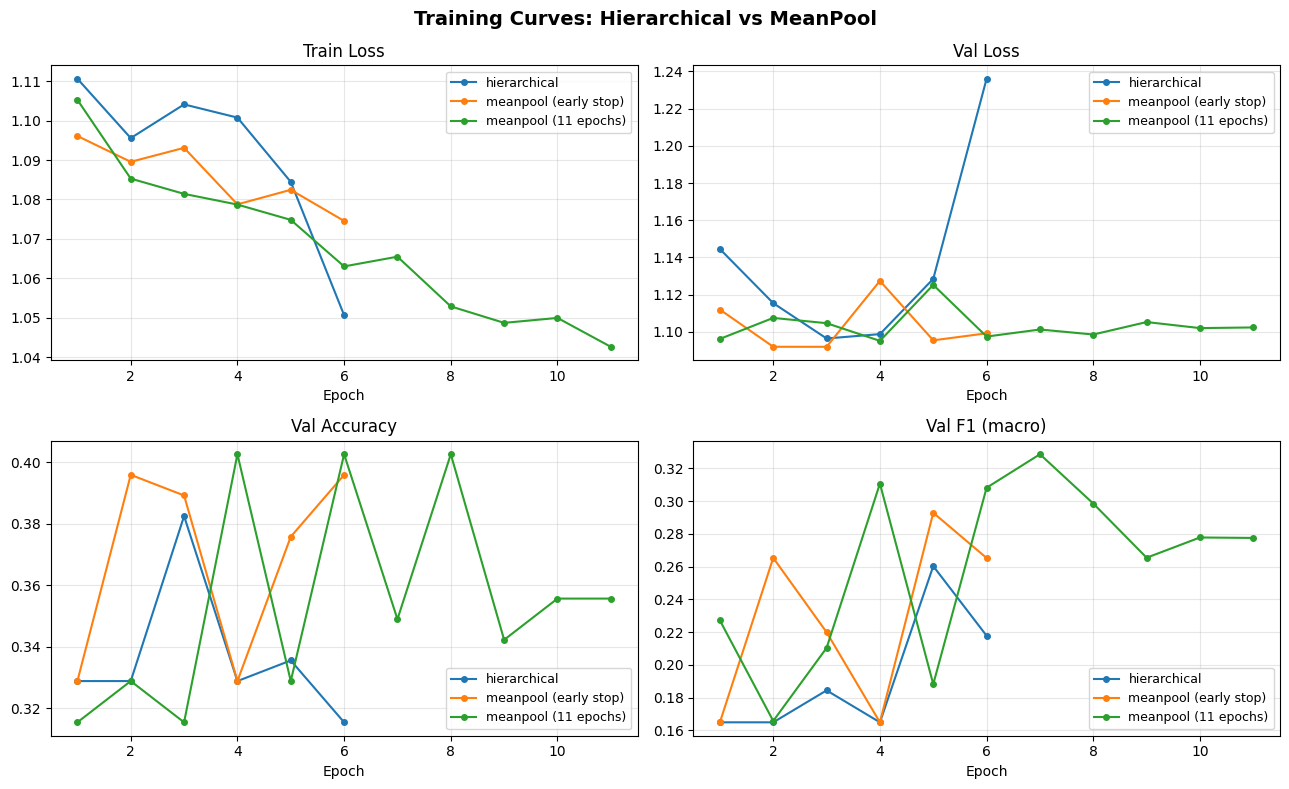
\includegraphics[width=0.95\textwidth]{images/training_curves.png}
\caption{Training and validation loss curves, validation accuracy, and validation macro F1 for the FinBERT mean-pooling baseline and the hierarchical transformer. These curves should be used to discuss underfitting, overfitting, and model selection.}
\label{fig:loss-curves}
\end{figure}

\begin{figure}[H]
\centering
\fbox{\parbox{0.68\textwidth}{\centering TODO: Insert final confusion matrix.}}
\caption{Confusion matrix for the final selected model. Rows should represent true labels and columns should represent predicted labels.}
\label{fig:confusion-matrix}
\end{figure}

\section{Discussion}

The main interpretation will depend on the final metrics, but the task should be evaluated carefully because stock returns are very noisy labels. If the hierarchical transformer improves macro F1 over mean pooling, that would suggest that cross-chunk attention helps the model use long transcript structure more effectively. If the improvement is small or negative, that would still be a meaningful result because it would show that extra model complexity does not necessarily create a stronger financial signal.

When analyzing the loss curves, we will look for the same patterns discussed in class. If training and validation loss are both high, the model is likely underfitting or the transcript text alone may not contain enough signal. If training loss decreases while validation loss rises, the model is overfitting, which is plausible because transformer models have many parameters compared with the number of labeled earnings calls. In that case, more regularization, more data, or additional structured financial features may be needed.

The main limitation is that transcripts alone do not capture investor expectations. A positive-sounding earnings call can still lead to a negative return if the market expected even better results. Future work could add earnings surprise, revenue surprise, sector, market capitalization, prior momentum, analyst estimates, volatility, and different return windows. We could also add interpretability tools that identify which transcript chunks most influenced the prediction.

\section{Safety, Security, and Ethics}

If deployed at scale, this model poses financial risks, as users may treat predictions as investment advice despite being trained on noisy data that may not generalize. Incorrect predictions could lead to losses, especially if a user interprets the output probabilities as certainty. There are also fairness concerns. Larger companies have more consistent transcripts and more liquid stock prices, so the model may work better for large firms than for smaller companies. The model could also learn superficial wording patterns rather than causal signals.n when the true driver was already known to the market. Any deployment should include clear disclaimers and monitoring, and the model should not be used as a standalone trading system. In this project, we treat the model as a research and learning tool for financial NLP, not as a production-ready trading model.
\section{Conclusion}

This project applies deep learning methods from the course to a real-world long-document NLP problem. We built a pipeline for earnings call transcript classification, created a return-based three-class learning problem, implemented a FinBERT mean-pooling baseline, and added a hierarchical transformer to model relationships across transcript chunks. The final step is to insert training curves, test metrics, and error analysis after the remaining experiments are complete. Overall, the project shows how transformer models can be adapted to financial text while also showing why financial prediction is a difficult and high-risk domain.

\newpage
\appendix
\section{Appendix}

\subsection{Repository and Presentation Links}
\textbf{GitHub repository:} TODO: insert repository link. \\
\textbf{Presentation recording:} TODO: insert presentation recording link. \\
\textbf{Demo link:} TODO: insert HuggingFace Spaces or demo recording link, if used.

\subsection{Final Items to Insert Before Submission}
\begin{itemize}
    \item Final train/validation/test counts after return filtering.
    \item Class balance table for down, flat, and up labels.
    \item Baseline and hierarchical model training curves.
    \item Final test metrics: accuracy, macro F1, weighted F1, up F1, and down F1.
    \item Confusion matrix and two to three sentence error analysis.
    \item Final result sentence in the abstract and conclusion.
\end{itemize}

\subsection{Team Contributions}

\textbf{Nikita Mehendale: Data pipeline.} Collected and normalized earnings call transcripts, downloaded stock and SPY return data, and implemented return-based label construction.

\textbf{Person 2: Preprocessing and dataset.} Implemented transcript tokenization, chunking, attention masks, caching, the PyTorch dataset class, and chronological train/validation/test loaders.

\textbf{Person 3: FinBERT baseline.} Implemented the FinBERT chunk encoder, partial layer freezing, mean-pooling baseline, and baseline classification head.

\textbf{Prabhav Pagadala: Hierarchical transformer.} Implemented the advanced hierarchical transformer with chunk-level positional embeddings, a learnable transcript-level \texttt{[CLS]} token, self-attention across chunks, and final classification head.

\textbf{Patrick Phan \& 6: Training, evaluation, and demo.} Implemented the training loop, AdamW optimization, gradient clipping, learning rate scheduling, early stopping, W\&B logging, evaluation metrics, checkpoint saving, and Gradio demo structure.
\end{document}
